\documentclass[10pt,a4paper,twocolumn]{article}

% Packages (alphabetical order)
\usepackage{amsmath,amssymb}
\usepackage{balance}
\usepackage{booktabs}
\usepackage{caption}
\usepackage[margin=17mm]{geometry}
\usepackage{graphicx}
	\graphicspath{
		{./}
		{../graphics/}
	}
\usepackage{hyperref}
\hypersetup{
  	bookmarks=true,
    unicode=false,
    pdftoolbar=true,
    pdfmenubar=true,
    pdffitwindow=true,
    pdftitle={Multi-agent systems},
    pdfauthor={},
    pdfsubject={},
    pdfnewwindow=true,
    pdfkeywords={},
    colorlinks=true,
    linkcolor=blue,
    citecolor=blue,
    filecolor=blue,
    urlcolor=blue
}
\usepackage{lipsum}
\usepackage{microtype}
\usepackage[numbers,sort&compress]{natbib}
	\bibliographystyle{apalike2}

% Title information
\title{Stigmergic Coordination in UAV Search and Rescue:\\A Behavioral Sensitivity Analysis}
\author{
  Arthur Schauwvlieghe \\
  {\small KU Leuven} \\
  \texttt{arthur.schauwvlieghe@student.kuleuven.be}
  \and
  Guust Delbaere \\
  {\small KU Leuven} \\
  \texttt{guust.delbaere@student.kuleuven.com}
  \and
  Harun Kalkanci \\
  {\small KU Leuven} \\
  \texttt{harun.kalkanci@student.kuleuven.be}
}
\date{}

\begin{document}
\maketitle

\begin{abstract}
Efficient search and rescue in large, unknown environments remains a fundamental challenge for autonomous systems. We present a multi-agent model of UAV-based search and rescue that combines Belief-Desire-Intention (BDI)-inspired statechart reasoning with a reversed Ant Colony Optimization (ACO) mechanism. Rather than following pheromone trails toward rewarding locations, agents treat pheromone as a collective spatial memory of recently covered ground and actively avoid it. A secondary stigmergic signal (victim detection) acts as a positive attractor, creating a dynamic Explore--Exploit balance that requires no centralized scheduling. We encode agent behavior in a hierarchical statechart that makes every behavioral transition explicit and auditable, enabling meaningful sensitivity analysis. We describe the full implementation in AnyLogic, including the victim placement model, pheromone grid, and battery management logic, and present an automated experimental pipeline for parameter sweeps. Our results characterize how the ACO scoring exponents, step length, and candidate count jointly shape the convergence speed and reliability of the swarm.
\end{abstract}

% ─────────────────────────────────────────────────────────────────────────────
\section{Introduction}
% ─────────────────────────────────────────────────────────────────────────────

Search and rescue (SAR) operations rank among the most time-critical challenges that emergency services face. When a disaster strikes, whether a structural collapse, a flooding event, or a wildfire, the probability of survival decreases sharply with elapsed time, placing enormous pressure on how quickly rescuers can locate and extract victims~\citep{bk:Wooldridge2009}. Ground-based response teams, while effective, are slow to deploy, constrained by terrain, and themselves vulnerable to the same hazards that endanger victims. Unmanned Aerial Vehicles (UAVs) offer a compelling alternative: they can be airborne within minutes, traverse difficult terrain without risk to human personnel, and cover large areas at speeds that ground teams cannot match.

The central engineering challenge of a multi-UAV search mission is coordination. A single UAV has severely limited coverage capacity. A fleet of independent agents, each acting without regard to the others, will duplicate effort over some areas while leaving others entirely unsearched. Classical solutions rely on centralized task allocation: a ground station partitions the search space, assigns sectors to individual UAVs, and updates assignments as the mission evolves. This architecture is fragile in disaster environments where communication links are unreliable, the controller itself is a single point of failure, and the computational burden of replanning grows with fleet size.

Decentralized multi-agent systems (MAS) offer a more resilient alternative. By encoding coordination into local behavioral rules and shared environmental cues, a fleet achieves coherent global search patterns without any agent requiring a global view or receiving a central directive. This approach, inspired by the collective intelligence of social insects, is robust to individual agent failure, scales naturally with fleet size, and requires no explicit inter-agent communication~\citep{bk:Bonabeau1999}.

This paper presents a compact, interpretable model of decentralized UAV-based SAR implemented in AnyLogic. The model rests on two design principles. First, UAVs coordinate through a reversed Ant Colony Optimization (ACO) mechanism. Pheromone marks recently covered ground and repels future agents, guiding the swarm toward unexplored territory. Second, each UAV encodes its decision logic in a Belief-Desire-Intention (BDI)-inspired statechart that makes every behavioral mode and transition condition explicit. This transparency is essential for meaningful sensitivity analysis.

Our contributions are threefold. We design and implement a complete agent-based SAR model with three interacting agent types. We formalize the reversed ACO scoring function and the dual stigmergic mechanism that governs the Explore--Exploit balance. Finally, we construct an automated experimental pipeline that performs a systematic grid search over the model's key behavioral parameters, enabling a rigorous characterization of how local movement rules shape global search performance.

% ─────────────────────────────────────────────────────────────────────────────
\section{Background}
% ─────────────────────────────────────────────────────────────────────────────

\subsection{Agent-Based Modelling and Multi-Agent Systems}

Agent-based modelling (ABM) studies complex systems by simulating the behaviors and interactions of individual autonomous agents, allowing emergent macro-level phenomena to arise from micro-level rules~\citep{ar:Macal2016,ar:GallegatiEtAl2024}. ABM is particularly well suited to domains where top-down analytical models fail: wherever emergence, adaptation, or heterogeneous populations play a central role. Reynolds' boids model~\citep{inpr:Reynolds1987} offered an early and influential demonstration of this principle: three local steering rules (separation, alignment, and cohesion) produce globally coherent flocking behavior that is visually indistinguishable from that of real birds.

In the context of SAR, ABM provides a natural framework for studying how simple agent-level behavioral rules translate into collective search coverage, and how sensitive that translation is to the specific parameter choices made by the system designer.

\subsection{Belief-Desire-Intention Architecture}

The BDI model formalizes the internal state of a rational agent as a triple. Beliefs represent what the agent knows about the world, desires represent the objectives it seeks to achieve, and intentions represent the plans it has committed to executing~\citep{bk:Wooldridge2009}. BDI agents are deliberative. They reason about beliefs to select intentions consistent with their desires. They are also reactive, meaning new perceptions update beliefs and changing circumstances can revise intentions.

Full BDI implementations can be architecturally complex. Our model adopts a distilled BDI perspective, encoding the essential belief-update and intention-selection logic directly in a hierarchical statechart. Sensor readings form the belief base, coverage of the search space is the standing desire, and the current commitment to a specific movement mode (exploring, exploiting, or charging) constitutes the intention. Every belief update and intention switch is a named, visible transition in the chart.

\subsection{Ant Colony Optimization and Stigmergy}

Stigmergy is a form of indirect coordination in which agents communicate through persistent modifications to a shared environment rather than through direct messaging~\citep{bk:Bonabeau1999}. ACO operationalizes this principle: artificial ants deposit pheromone on paths they traverse, biasing future agents toward high-pheromone routes through a positive feedback loop~\citep{bk:Dorigo2004}.

Classical ACO targets optimization problems where convergence toward a small set of high-quality solutions is the goal. Search coverage requires the opposite behavior: divergence. An agent drawn back toward a high-pheromone cell wastes effort on already-searched ground. Our model inverts the ACO reinforcement signal, using pheromone as a coverage record that repels rather than attracts. This inversion preserves the full mathematical apparatus of ACO (pheromone deposition, exponential evaporation, and probabilistic selection based on pheromone levels) while reversing its behavioral semantics. The result is a dispersion mechanism rather than a convergence mechanism.

% ─────────────────────────────────────────────────────────────────────────────
\section{Design Rationale}
% ─────────────────────────────────────────────────────────────────────────────

\subsection{Pheromone Repulsion}

The core insight driving our coordination mechanism is that pheromone, in the SAR context, carries the opposite semantic meaning from its classical ACO role. In standard ACO, high pheromone indicates a historically rewarding path, a quality signal that attracts future agents. In SAR, high pheromone on a grid cell simply means a UAV passed over it recently, a redundancy signal that should repel future agents.

By scoring candidate waypoints inversely with their pheromone level, we ensure that the swarm collectively avoids recently covered ground and moves toward less-explored territory. As pheromone evaporates over time, previously covered cells gradually regain attractiveness, reflecting the fact that conditions may have changed or that a victim may have been missed on an earlier pass. The evaporation rate therefore controls the time horizon of the swarm's spatial memory. A fast rate causes the swarm to quickly forget where it has been, enabling rapid re-coverage. A slow rate maintains longer-lasting coverage records at the cost of slower re-exploration of old areas.

\subsection{Explore and Exploit}

Repulsive pheromone is only one direction of stigmergic influence in our system. Victims provide the complementary signal: attraction. When a victim enters the forward sensor cone of a UAV, the detection immediately triggers a behavioral switch that overrides the exploratory trajectory. The UAV commits to an approach and flies directly toward the target.

The two signals together create a complete Explore--Exploit dynamic without any explicit scheduling mechanism. In the absence of detections, repulsive pheromone pushes agents outward into unsearched space. On detection, attractive victim signals pull individual agents inward toward a specific target. After confirming a victim, a brief local search phase biases the confirming UAV toward the victim's vicinity. This exploits the spatial clustering of the victim distribution. If additional victims are clustered nearby, the confirming agent is likely to discover them in the next few steps.

The swarm thus adapts its collective behavior, oscillating between broad coverage and focused exploitation, through purely local stigmergic signals with no global state and no communication between agents beyond the shared pheromone grid.

\subsection{Transparent Behavior}

A stated requirement of this work is that the model's behavior be understandable and its sensitivity patterns be interpretable, not merely measured. An opaque reactive controller might achieve higher raw performance, but it would offer no insight into which features of the behavior drive observed differences, the very insight that a sensitivity analysis aims to extract.

Our solution is a hierarchical BDI-inspired statechart in which every behavioral mode is a named state and every decision is an explicit, labeled transition. The statechart reads as a behavioral specification: given the current state and a set of observable conditions, the next state is deterministic and visible. This transparency serves two purposes. First, it lets the experimenter reason about expected behavior before running any experiment. Second, it enforces a clean design discipline. Each state handles exactly one responsibility, transitions carry explicit conditions, and the overall organization reflects the MAS principle of decentralized, structured agency. The resulting system is easier to debug, explain, and extend, even if it does not provide mechanical formula-level tracing from a single parameter change to a specific output difference.

\subsection{Victim Placement}
\label{sec:design_victim}

Real disaster scenarios rarely produce uniformly distributed victims. Structural collapses, vehicle accidents, and flooding events tend to create spatial clusters, groups of victims concentrated in the area of maximum impact. A uniform victim distribution would favor strategies with high spatial uniformity and would not expose the Explore--Exploit tension that is central to our design.

We model victim placement with a Gaussian Mixture Model (GMM). At the start of each run, cluster centers are drawn uniformly from the search space, and victims are sampled from the mixture distribution defined by those centers, their relative weights, and per-cluster spread parameters. This produces realistic clustering while remaining analytically tractable and configurable. The number of clusters, their probabilities, and their spatial spreads can be varied to test robustness across scenarios ranging from a single concentrated incident to a broadly dispersed multi-site disaster.

% ─────────────────────────────────────────────────────────────────────────────
\section{System Model}
% ─────────────────────────────────────────────────────────────────────────────

\subsection{Simulation Environment}

The simulation environment is a two-dimensional continuous space of $45 \times 25$ meters, representing a bounded search area. We overlay the space with a shared pheromone grid of $90 \times 50$ cells, each covering a $0.5 \times 0.5$ meter area. This grid is the primary medium of stigmergic coordination: it accumulates pheromone from all UAVs and each UAV queries it at every planning step. By default, the simulation runs two UAV agents and five Victim agents. A charging station sits at the bottom right of the search area.

\subsection{Victim Agent}

The Victim agent is a passive data container with no behavioral logic of its own. Each instance holds a spatial position assigned at initialization by the Main agent, and three state variables: a flag indicating whether the victim has been found, the index of the discovering UAV, and the simulation time of discovery. The Victim agent takes no actions and responds to no events. All victim logic (placement, discovery marking, and logging) runs in the Main agent, while the UAV agent handles sensing and confirmation.

\subsection{Main Agent}

The Main agent serves as the simulation orchestrator. At initialization it performs three tasks: seeding the random number generator for full reproducibility, computing an evenly-spaced dispersal position for each UAV along the horizontal midline, and placing victims by sampling from the configured GMM.

The Main agent is the sole owner of the pheromone grid. Pheromone decays continuously according to an exponential model:
\begin{equation}
    \tau(t) = \tau_0 \cdot e^{-\rho\,(t - t_0)},
    \label{eq:evaporation}
\end{equation}
where $\tau_0$ is the deposited level recorded at reference time $t_0$ and $\rho$ is the evaporation rate. To avoid recomputing decay at every time step, the grid uses lazy evaluation. Each cell stores its last-deposited value and the timestamp of that deposit, and the current effective level is computed on demand by applying Equation~\eqref{eq:evaporation} at query time. This requires no background event for evaporation.

When a UAV confirms a victim, the Main agent marks the nearest Victim instance as found and resets the pheromone to zero in a fixed radius around the confirmed location. It also appends an event record to a comma-separated values (CSV) log. This local reset opens the victim's vicinity for re-examination, which is useful under a clustered victim distribution. When all victims have been confirmed, the Main agent records the convergence time and terminates the simulation. A safety-stop event enforces a configurable time limit, recording a timeout result for any run that has not converged.

\subsection{UAV Agent}
\label{sec:uav}

Each UAV runs the hierarchical statechart shown in Figure~\ref{fig:statechart}. The chart has three primary top-level modes: \textsc{Startup}, \textsc{Explore}, and \textsc{Exploit}, together with a \textsc{ChargingStation} mode that the UAV can enter from either \textsc{Explore} or \textsc{Exploit} at any time. A concurrent orthogonal state, \textsc{BatteryDischarge}, runs in parallel throughout the mission and continuously depletes the battery during flight.

\subsubsection{Startup}

At simulation start all UAVs share a common launch point. The \textsc{Startup} mode immediately moves each UAV to its pre-assigned dispersal position. The dispersal positions are evenly spaced so that the fleet enters the search space with minimal initial pheromone overlap. Sensing is active during the dispersal flight: a victim detected en route causes an immediate transition to \textsc{Exploit} without waiting for dispersal to complete. Once the UAV arrives at its dispersal target, \textsc{Startup} exits unconditionally and the main behavioral cycle begins in \textsc{Explore}.

\subsubsection{Explore}

The \textsc{Explore} mode implements the reversed ACO coverage cycle. As shown in Figure~\ref{fig:statechart}, it cycles through four sub-states: \textsc{ExploreSense}, a branch node \textsc{ExploreAdaptStep}, \textsc{ExplorePlan}, and \textsc{ExploreMove}. The central idea is that at each planning cycle the UAV considers $n$ candidate waypoints arranged in a ring at distance $d$ from its current position.

\paragraph{ExploreSense.}
On every sensing tick (at 2\,Hz), the UAV sweeps a forward-facing field-of-view (FOV) cone over the area ahead of it. Any unfound victim that falls within the cone's angular extent and within sensor range triggers a detection signal. The UAV also records which grid cells the cone covers. It deposits pheromone into each of those cells and stamps them with the current time as their last-sensed timestamp, building up a shared spatial memory of where the swarm has already looked. Finally, it reads the pheromone level at each of the $n$ candidate positions on the planning ring and stores the minimum value $\tau_{\min}$, which feeds into the adaptive step check.

\paragraph{ExplorePlan.}
To choose a waypoint, the UAV scores each of the $n$ candidate positions on the planning ring. As shown in Figure~\ref{fig:simulation}, these candidates appear as yellow dots evenly spaced on a circle around the UAV, and the selected waypoint is marked in red. Each candidate $i$ receives a score:
\begin{equation}
    s_i \;=\; \left(\frac{1}{1 + \tau_i}\right)^{\!\alpha} \cdot \eta_i^{\,\beta},
    \label{eq:aco}
\end{equation}
where $\tau_i$ is the effective pheromone at the candidate's cell (from Eq.~\eqref{eq:evaporation}), $\eta_i = \max(0, 1 - f_i)$ is the cell's staleness, and $f_i$ is its freshness:
\begin{equation}
    f_i(t) \;=\; \max\!\left(0,\;1 - \frac{t - t_{\mathrm{last},i}}{T_{\mathrm{stale}}}\right).
    \label{eq:freshness}
\end{equation}
A cell sensed just moments ago has $f_i \approx 1$ and $\eta_i \approx 0$, while a cell not sensed for $T_{\mathrm{stale}}$ seconds has $f_i = 0$ and $\eta_i = 1$. The exponent $\alpha$ weights the pheromone repulsion term and $\beta$ weights the staleness attraction term. Candidates that fall within the collision-avoidance radius of another UAV receive a strong score penalty, discouraging clustering. The UAV then draws a waypoint by sampling from a probability distribution formed by normalizing the scores across all candidates. This preserves behavioral diversity while biasing movement toward low-pheromone, stale cells.

\paragraph{ExploreAdaptStep.}
Before executing the plan above, a branch node checks whether $\tau_{\min}$ exceeds a configurable threshold. When this threshold is exceeded, every candidate on the ring already lies in well-covered territory. The UAV has thoroughly explored its immediate neighborhood and cycling through the same candidate ring would add little new coverage. In this case, the UAV scales up its step radius for the coming planning cycle:
\begin{equation}
    d_{\mathrm{current}} = d \cdot \min\!\left(M,\; 1 + \tau_{\min}\right),
    \label{eq:adaptstep}
\end{equation}
where $d$ is the base step length and $M$ is the configurable maximum multiplier (default $M = 2$). Enlarging the candidate ring lets the UAV escape the saturated neighborhood and reach fresher, less-covered territory beyond it.

\paragraph{ExploreMove.}
The UAV flies directly toward the selected waypoint, the red dot in Figure~\ref{fig:simulation}. Sensing continues at 2\,Hz throughout the flight: if a victim enters the FOV cone at any point mid-trajectory, the UAV immediately transitions to \textsc{Exploit} without waiting to reach the waypoint. This transition is visible in Figure~\ref{fig:simulation}, where UAV1's orange FOV cone indicates an active victim detection. On arrival at the waypoint, the cycle returns to \textsc{ExploreSense}.

\subsubsection{Exploit}

\textsc{Exploit} is entered whenever a sensing operation detects a victim above the confidence threshold. The three sub-states, described here in execution order as shown in Figure~\ref{fig:statechart}, form a confirm-and-loop cycle.

\paragraph{ExploitVerify.}
The UAV continues sensing at 2\,Hz to confirm that the detected signal persists before committing to a physical approach. In our current implementation the sensor model is deterministic and fully accurate within its detection radius, so transient false positives cannot occur and this sub-state is functionally redundant. It is nonetheless included so the architecture generalizes cleanly to probabilistic sensor models where spurious detections are a genuine concern.

\paragraph{ExploitApproach.}
Once a stable detection is confirmed, the UAV flies directly to the target's sensed coordinates. Movement speed is the same as during exploration, with the only difference being that the destination is a victim location rather than a scored candidate waypoint.

\paragraph{ExploitConfirm.}
On arrival at the target, the UAV reports the confirmed discovery to the Main agent, which marks the victim, clears the local pheromone, and logs the event. The UAV then enters a local search mode, biasing its next several waypoint selections toward the confirmed location. This local bias is motivated directly by the GMM victim placement model described in Section~\ref{sec:design_victim}. Because victims cluster spatially around shared incident centers, confirming one victim makes nearby locations disproportionately likely to hold additional victims, and the local bias lets the UAV capitalize on that structure. Detection state is then reset and the loop returns to \textsc{ExploitVerify} to scan for additional nearby victims. If confidence remains below the threshold after the reset, the top-level condition routes the UAV back to \textsc{Explore}.

\subsubsection{ChargingStation and Battery Management}

A concurrent orthogonal statechart (\textsc{BatteryDischarge}) continuously depletes the battery at a constant rate during all non-charging flight. When the battery level drops below a configurable return threshold (default 20\%), a top-level transition preempts any ongoing mode, saves the UAV's current position, and routes it to \textsc{ChargingStation}.

Within \textsc{ChargingStation}, the \textsc{MovingToCharger} sub-state navigates the UAV to the charging station. During this transit, all non-essential operations are suspended: sensing stops, pheromone deposits stop, and the UAV focuses solely on reaching the charger. With only movement active, the battery drains more slowly than during full exploration. The \textsc{Charging} sub-state then replenishes the battery at a fixed rate until it is fully charged. On completing a charge cycle, the waypoint planner uses the saved pre-charge position as a return target, so the UAV resumes its coverage mission from approximately where it was interrupted, limiting the coverage gap introduced by the battery return.

% ─────────────── full-width statechart figure ─────────────────────────────
\begin{figure*}[ht]
    \centering
    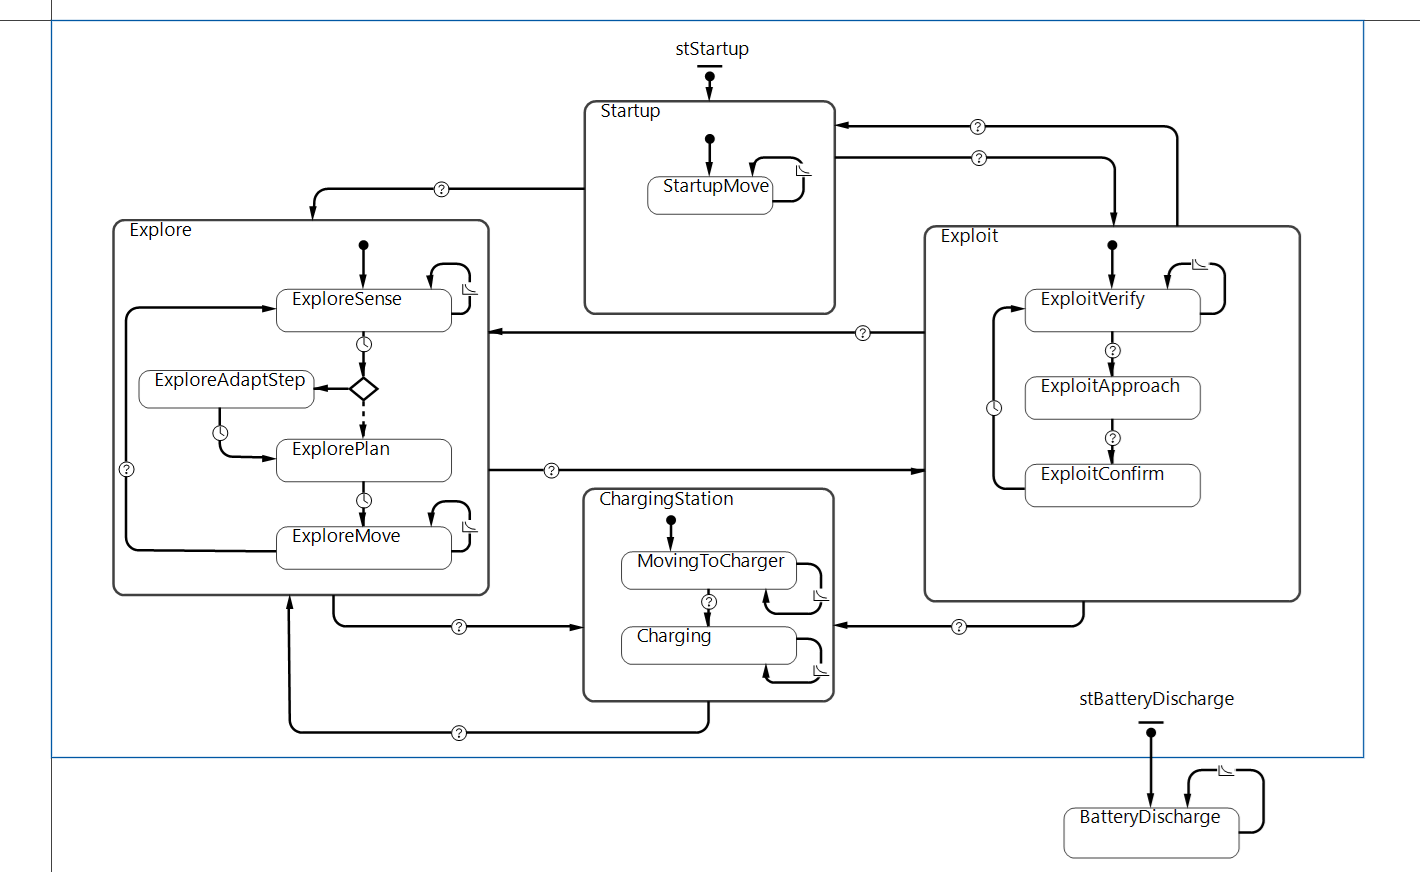
\includegraphics[width=\textwidth]{img/statechart.png}
    \caption{The BDI-inspired UAV statechart. The three primary modes, \textsc{Startup}, \textsc{Explore}, and \textsc{Exploit}, are shown with their internal sub-states and transitions. \textsc{ChargingStation} can be entered from either \textsc{Explore} or \textsc{Exploit} on a low-battery condition. The concurrent \textsc{BatteryDischarge} state (bottom right) runs orthogonally to all other modes.}
    \label{fig:statechart}
\end{figure*}

% ─────────────────────────────────────────────────────────────────────────────
\section{Experimental Setup}
% ─────────────────────────────────────────────────────────────────────────────

To characterize how search performance responds to the model's key behavioral parameters, we run two complementary experiments using AnyLogic's built-in sweep infrastructure, with sensor range fixed at 5 meters. The first sweeps all four parameters in a full factorial grid to expose their joint interactions. The second holds three parameters at their defaults and varies only one at a time, isolating the individual effect of each parameter in turn.

\textbf{Candidate count} ($n$) controls the angular resolution of the waypoint selection ring: more candidates offer a finer-grained directional choice and a smoother score distribution, at the cost of additional scoring operations per planning step. We vary $n \in \{12, 18, 24, 30, 36\}$.

\textbf{Step length} ($d$) sets the radius of the candidate circle in meters, determining how far the UAV moves at each planning step. Longer steps increase the rate of area coverage but reduce spatial resolution and the ability to target specific nearby cells precisely. We vary $d \in \{50, 75, 100, 125, 150\}$\,m.

\textbf{Pheromone exponent} ($\alpha$) controls the weight of the pheromone repulsion term in Equation~\eqref{eq:aco}. A higher value makes the scoring function more sensitive to pheromone differences, producing stronger and more decisive avoidance of recently covered cells. We vary $\alpha \in \{0.5, 1.0, 1.5, 2.0, 2.5\}$.

\textbf{Staleness exponent} ($\beta$) controls the weight of the cell-age term. A higher value gives stronger preference to cells that have not been sensed recently. We vary $\beta \in \{1.0, 1.5, 2.0, 2.5, 3.0, 3.5, 4.0\}$. In practice, because our pheromone evaporation rate is kept very low and victims do not move, recently explored cells never become genuinely stale and $\beta$ has limited impact on outcomes.

We evaluate each parameter combination across 10 independent random seeds. The seed determines both the victim placement (GMM sampling) and the stochastic choices in waypoint selection. Replicating across seeds ensures that observed performance differences reflect genuine parameter sensitivity rather than idiosyncrasies of a particular victim configuration.

We record two primary metrics per run. \textbf{Convergence time} is the simulation time at which the last victim is confirmed found. \textbf{Convergence rate} is the fraction of runs for a given parameter configuration in which all victims are found before the 200-second safety-stop limit. Runs that time out are recorded with an undefined convergence time and reduce the convergence rate of their configuration. The dual-metric approach distinguishes configurations that are consistently fast from those that succeed on only some seeds, an important distinction for evaluating robustness.

The experimental pipeline is fully automated. Each run writes its result incrementally to a CSV log file in a numbered experiment folder, allowing runs to proceed in parallel without coordination beyond synchronized file writes. When all runs complete, a Python post-processing script picks up the CSV files automatically and produces the full set of visualizations without manual intervention. A snapshot of the running simulation, illustrating the pheromone grid, UAV sensor cones, and victim locations, is shown in Figure~\ref{fig:simulation}.

% ─────────────── full-width simulation figure ─────────────────────────────
\begin{figure*}[ht]
    \centering
    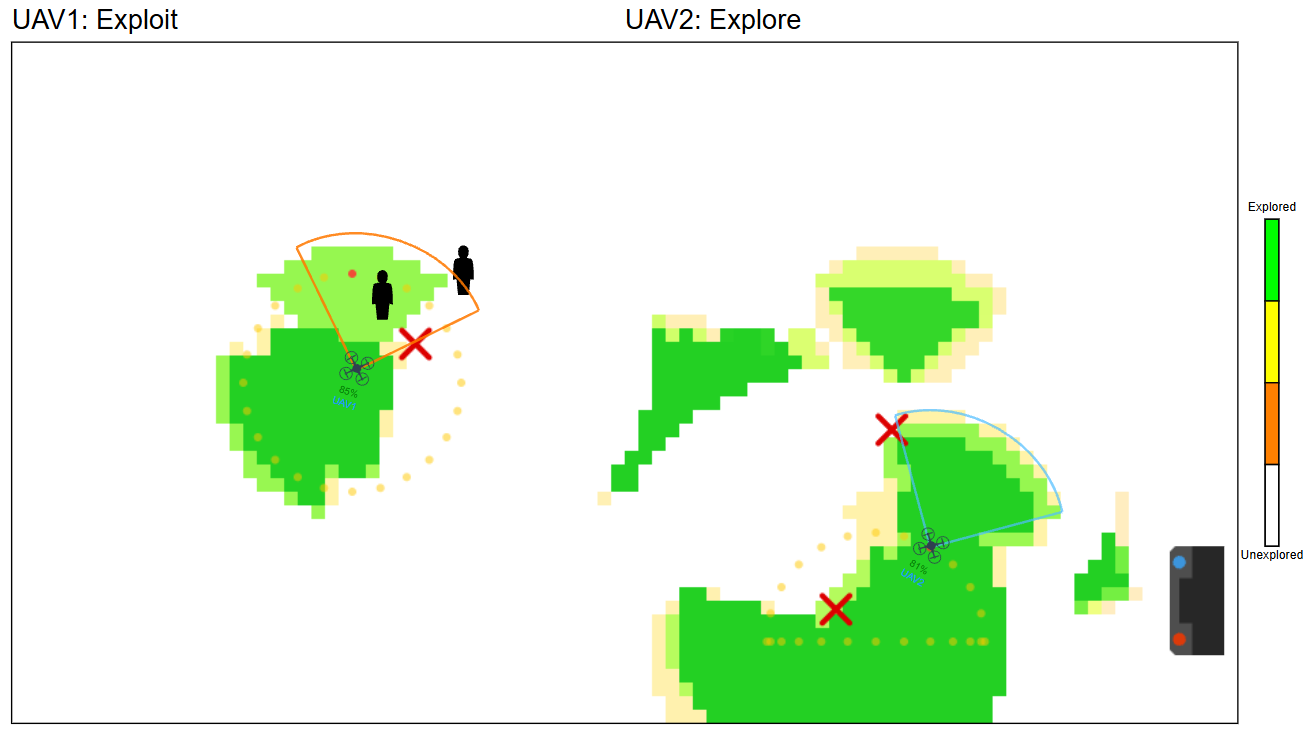
\includegraphics[width=\textwidth]{img/simulation.png}
    \caption{A snapshot of the running simulation. The heat-map overlay shows the current pheromone distribution: green tones indicate high coverage intensity and white indicates unexplored territory. UAV2 (right) is in \textsc{Explore} mode: its blue FOV cone sweeps the area ahead, yellow dots show the $n$ candidate waypoints on the planning ring, and the red dot marks the selected destination. UAV1 (left) is in \textsc{Exploit} mode: the orange FOV cone indicates an active victim detection in progress. Red crosses mark already-confirmed victims.}
    \label{fig:simulation}
\end{figure*}

% ─────────────────────────────────────────────────────────────────────────────
\section{Results and Discussion}
% ─────────────────────────────────────────────────────────────────────────────

One implementation choice shapes all the results: in our simulation, victims are stationary and do not change location after placement. Because the underlying search objective does not change, we set the pheromone evaporation rate to a very low value. Pheromone deposited on a cell effectively persists for the duration of a run, making recently explored territory reliably repulsive. This also explains why the staleness exponent $\beta$ has little measurable effect: cells never genuinely become stale when the state of the world does not change beneath them.

\lipsum[1-2]

\lipsum[3-4]

\lipsum[5-6]

% ─────────────────────────────────────────────────────────────────────────────
\section{Conclusion}
% ─────────────────────────────────────────────────────────────────────────────

We present a decentralized model of UAV-based search and rescue combining BDI-inspired statechart reasoning with a reversed ACO coordination mechanism. The design deliberately prioritizes interpretability alongside performance: every behavioral mode is a named state, every transition carries an explicit condition, and the coordination mechanism reduces to a single scoring formula. The statechart structure makes the system auditable in a way that a monolithic controller cannot offer. Each state handles exactly one responsibility and the overall organization reflects the MAS design principle of decentralized, structured agency. This makes the system easier to reason about, explain, and debug, even if it does not provide mechanical formula-level tracing from a single parameter change to a specific output difference.

\lipsum[7]

The model's simplifications define the boundaries of its validity. The environment is obstacle-free and two-dimensional. Real terrain constrains UAV trajectories in ways the model does not capture. The sensor is idealized, providing binary detection within a clean geometric cone with no noise, no false positives, and no occlusion. Coordination runs entirely through the shared pheromone grid, which presupposes a lossless shared data structure rather than an explicit radio channel. Victim positions are static. These simplifications are deliberate: they isolate the behavioral mechanisms of interest from confounding physical factors. But they establish the ceiling on the model's direct applicability.

Extending the model toward real-world deployment would require addressing each of these gaps. A probabilistic sensor model would replace the binary threshold with a Bayesian confidence update, accumulating evidence over multiple sensor passes and supporting partial detections. The shared pheromone grid would become a distributed gossip protocol. Each UAV would maintain a local copy and periodically merge it with neighbors within radio range, introducing communication latency and network partitions as new performance variables. Battery management would need hardware-specific discharge curves that account for wind, payload, and temperature. Regulatory constraints (altitude limits, beyond-visual-line-of-sight certification, and mandated collision avoidance margins) would impose hard trajectory constraints beneath the statechart layer.

Despite these gaps, the core design principles validated here transfer cleanly to more physically realistic architectures. Repulsive stigmergy for coverage dispersion, attractive stigmergy for exploitation, and a transparent statechart for inspectable behavioral switching are not artifacts of the simplified model. They are general principles applicable to any representation of recently-searched space, any detection model that produces a confidence signal, and any behavior architecture that supports explicit state modelling. The sensitivity analysis framework developed here provides a methodology that can be carried forward to guide calibration as the model is progressively extended toward deployment.

\balance
\bibliography{Bib.bib}

\end{document}
